\documentclass{article}
\usepackage{xeCJK}
\setmainfont{KaiTi}

\begin{document}
\tableofcontents
\newpage

\section{ORBSLAM}
ORBSLAM的总体框架如图(\ref{fig:orbslam_overview})所示.
\begin{figure}
	\centering
	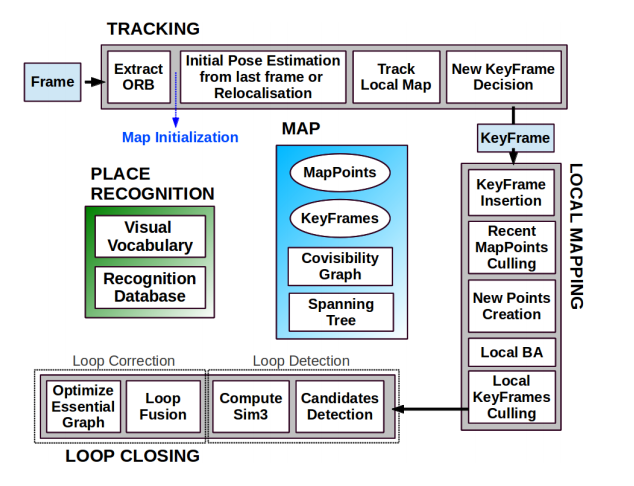
\includegraphics[width=14cm]{images/orbslam_overview.png}
	\label{fig:orbslam_overview}
	\caption{ORBSLAM总体框架}
\end{figure}

\section{地图初始化}
地图初始化是单目相机必须具备的步骤,因为单张图像不能够回复地图点的深度信息.单目地图初始化的方法一般由两种:(1)假设局部为平面,利用单应性恢复相机相对位姿;(2)计算本征矩阵.这篇文章使用的方法是在平面的单应性和非平面的基本矩阵之间自动选择.(这一部分暂时不讲)

\section{跟踪}
当相机每接收到新的帧时,需要运行跟踪线程.相机位姿的优化,包含了$motion-only \quad BA$.
\subsection{ORB提取}
在尺度因子为$1.2$的$8$层上提取FAST角点,对于$512\times 384$到$752\times 480$的分辨率,提取$1000$个角点.为了保证角点均匀分布,在每一层上将图像分为均匀的网格,并且在每个网格中提取至少$5$个角点.

\subsection{初始位姿估计}
如果上一帧跟踪成功,则使用恒速模型来预测相机的位姿并且对上一帧观测到的地图点进行引导性的搜索.如果没有找到足够的匹配点(比如运动模型被严重破坏),进行宽搜索.然后使用找到的匹配点进行优化.

\subsection{全局重定位的初始位姿估计}
如果跟踪失败了,将当前帧转换成视觉词袋并在识别数据库中查找全局重定位的候选关键帧.在每一帧中计算$ORB$对应的,然后使用$RANSAC$方法和$PnP$算法求对应的位姿.如果找到足够多的内点,
\section{局部构图}

\section{场景识别}

\section{闭环检测}
\subsection{查询数据库}
首先将当前帧转换成$bag-of-word$向量$v_t$,并在数据库中查询最相似的$bag-of-words$向量集,


\begin{appendix}
BA(Bundle Adjustment)作为SLAM中的重要的概念,必须要弄清楚.地图点的三维位置$X_{w,j}\in R^3$和关键帧位姿$T_{iw}\in SE(3)$,其中$w$代表世界坐标系(即地图点在世界坐标系中表示),通过最小化相对于匹配点$x_{i,j}\in R^2$的重投影误差来优化.地图点$j$在关键帧$i$中的观测误差为
$$e_{i,j}=x_{i,j}-\pi_i(T_{iw},X_{w,j})$$	
其中$\pi_i$是投影方程
$$
\begin{array}{c}
\pi_i(T_{iw},X_{w,j})=
\left[
\begin{array}{c}
	f_{i,u}\frac{x_{i,j}}{z_{i,j}}+c_{i,u} \\
	f_{i,v}\frac{y_{i,j}}{z_{i,j}}+c_{i,v}
\end{array}
\right] \\

[x_{i,j}\quad y_{i,j}\quad z_{i,j}]^T = R_{iw} X_{w,j}+t_{iw}
\end{array}
$$

待优化的代价函数为
$$
C=\sum_{i,j}\rho_h(e_{i,j}^T\Omega_{i,j}^{-1}e_{i,j})
$$
其中$\rho_h$为$Hubber$鲁邦代价函数,$\Omega_{i,j}=\sigma^2_{i,j}I_{2\times2}$的协方差矩阵.

在$full\quad
 BA$中(地图初始化使用了),优化所有的点和关键帧(第一帧除外,作为原点保持不变);在$local\quad BA$中,所有的地图点的位置进行优化,关键帧的位置保持不变;在位姿优化或$motion-only \quad BA$中,所有点的位置保持不变,只优化相机的位姿.
\end{appendix}
\end{document}

